\documentclass[prd,twocolumn,tightenlines,preprintnumbers,showpacs,superscriptaddress,notitlepage,nofootinbib,eqsecnum,floatfix,longbibliography]{revtex4}
\usepackage[utf8]{inputenc}
\usepackage[T1]{fontenc}
\usepackage{amsmath,amssymb}
\usepackage{bm,bbm}
\usepackage{graphicx}
\usepackage{color}
\usepackage{dsfont}

\usepackage{hyperref}
\hypersetup{
    colorlinks=true,       % false: boxed links; true: colored links
    linkcolor=blue,          % color of internal links
    citecolor=blue,        % color of links to bibliography
    filecolor=blue,      % color of file links
    urlcolor=blue           % color of external links
}

\begin{document}
\title{Solutions to Integer Programming from Quantum Annealing}

\author{Chia~Cheng~Chang}
\affiliation{RIKEN Interdisciplinary Theoretical and Mathematical Sciences (iTHEMS), Wako, Saitama 351-0198, Japan}
\affiliation{Department of Physics, University of California, Berkeley, California 94720, USA}
\affiliation{Nuclear Science Division, Lawrence Berkeley National Laboratory, Berkeley, California 94720, USA}
\author{Chih-Chieh~Chen}
\affiliation{R\&D Group, Grid Inc., Tokyo 107-0061, Japan}
\author{Christopher K\"orber}
\affiliation{Department of Physics, University of California, Berkeley, California 94720, USA}
\affiliation{Nuclear Science Division, Lawrence Berkeley National Laboratory, Berkeley, California 94720, USA}
\author{Travis~Humble}
\affiliation{Quantum Computing Institute, Oak Ridge National Laboratory, Oak Ridge, Tennessee 37831, USA}
\author{Jim~Ostrowski}
\affiliation{University of Tennessee}

\begin{abstract}
Abstract here...
\end{abstract}

\preprint{LLNL-JRNL-809712, RIKEN-iTHEMS-Report-20}

\maketitle
%%%%%%%%%%%%%%%%%%%%%%%%%%%%%%%%%
%%%%%%%%%%%%%%%%%%%%%%%%%%%%%%%%%
%%%%%%%%%%%%%%%%%%%%%%%%%%%%%%%%%
\tableofcontents

\flushbottom
\maketitle

\section{INTRODUCTION}
\label{sec:introduction}

Integer linear programming (ILP) is an integer optimization problem subject to inequality constraints and is a commonly tackled problem applicable to situations such as x~\cite{}, y~\cite{}, and z~\cite{}. In general however, ILP is classically NP-complete, and as a result, heuristic methods are employed~\cite{}. The NP-hardness of ILP can be understood by realizing that while the solution to an $n$-dimensional linear problem can be obtained in polynomial time, the optimal integer solution in general must be found in the $2^n$ integer solutions which surround the real number solution. Due to the importance and difficulty, in this work we present a method to obtain the optimal solution to ILP by employing methods of quantum annealing.

Quantum annealing solves a general quadratic binary optimization problem (QUBO) by slowly varying a time-dependent Hamiltonian~\cite{}. Through the adiabatic theorem of quantum mechanics, the annealer is prepared initially in a trivial ground state while the solution to ILP is encoded in the target Hamiltonian. Due to the explosion in research efforts towards hardware implementations of quantum annealers and future improvements to the annealing schedule~\cite{}, mapping ILP to QUBO provides a path forward towards obtaining optimal solutions to the class of integer optimization problems~\cite{2018Glover}.

Formally, ILP is defined as the optimization of a linear function
{\color{blue}
\begin{align}
f(x) = &\min\limits_{x}(\sum_i c_i x_i),\\
\textrm{subject to} \quad & \sum_i A_{ai}x_i +b_a \leq 0 \\
& x_i \geq 0,\\
& x_i \in \mathbb{Z}
\end{align}
}
where $i=1, \cdots,  N$ is the number of dependent variables and $a=1, \cdots, M$ the number of constraint equations. The inequality constraints can be rewritten as an equality by introducing slack variables $s$ such that the ILP becomes
{\color{blue}
\begin{align}
f(x) = &\min(\sum_i c_i x_i),\\
\textrm{subject to} \quad & \sum_i A_{a i}x_i + s_a + b_a = 0,\\
& s_a \geq 0,\\
& s_a \in \mathbb{Z},\\
& x_i \geq 0,\\
& x_i \in \mathbb{Z}.
\end{align}
}
Since quantum annealing solves the QUBO problem, we extend the proposed algorithm to solve integer quadratic optimization problems such that
{\color{blue}
\begin{align}
f(x) = \min\limits_{x}(\sum_{ij} x_i d_{ij} x_j + \sum_i c_i x_i)
\end{align}
}
without the introduction of auxiliary qubits.

{\color{red} Paragraph on how this is solved classically. Include strengths and drawbacks of classical solution.}

\section{RESULTS}
\label{sec:results}
We map integer variables $z_i$ to qubits under the following transformation~\cite{Chang:2018uoc}
\begin{align}
z_i = & \sum_{r=0}^{R_i-1} 2^r \psi_{ri}
\label{eq:int_to_bin}
\end{align}
where $\psi_{ri} \in \{0, 1\}$ while the number of qubits used to represent the $i$-th integer variable is allowed to vary with $R_i$. The transformation can in general be express as a rectangular matrix. For example, a vector of two integer variables $z_0$ and $z_1$ represented by one and two qubits respectively is given as
\begin{align}
\begin{pmatrix}
z_0\\
z_1
\end{pmatrix}
= &
\begin{pmatrix}
2^0 & 0 & 0\\
0 & 2^0 & 2^1
\end{pmatrix}
\begin{pmatrix}
\psi_{00}\\
\psi_{01}\\
\psi_{11}
\end{pmatrix}
\equiv T^z \begin{pmatrix}
\psi_{00}\\
\psi_{01}\\
\psi_{11}
\end{pmatrix}
\end{align}
The transformation can be reduced to a tensor product if $R_i$ is a constant for all $i$ such that
\begin{align}
\mathcal{R} = & \begin{pmatrix} 2^0 & \dots & 2^{R-1}\end{pmatrix},\\
\mathcal{Z} = & \begin{pmatrix} z_0 & \dots & z_{N-1}\end{pmatrix},\\
|\mathds{1}| = & |\mathcal{Z}|,\\
T^z = & \mathds{1}\otimes \mathcal{R}.
\end{align}

While the coefficients of the inequality constraints are not required to be integer valued, the inequalities can be trivially rescaled such that $s_i \in \mathbb{Z}$ given fixed precision coefficients $A_{ij}$ and $b_i$. As a result, we can restrict both $x_i$ and $s_i$ to sample over only positive integer values as allowed by Eq.~(\ref{eq:int_to_bin}).

\subsection{Integer Programming Mapping to QUBO}
\label{sec:results:ilp}
The integer quadratic optimization problem can be mapped to a minimization of the quadratic objective function
\begin{align}
\chi^2 = & \left[\Psi^x_{\mu} T^x_{\mu i}d_{ij} T^x_{j \nu}\Psi^x_\nu + c_i T^x_{i\mu} \Psi^x_\mu \right. \nonumber\\
&\left.+ p (A_{a b} T^x_{b \mu} \Psi^x_{\mu} + T^s_{a \alpha} \Psi^s_\alpha + b_a)^2 \right],\\
\Psi = & \begin{pmatrix}
\Psi^x\\
\Psi^s
\end{pmatrix},
\end{align}
where $p$ is the strength of the penalty factor which must be set large enough such that the constraints are satisfied under minimization. The objective function can be represented as a QUBO Hamiltonian
\begin{align}
E = &
\begin{pmatrix}
\Psi^x & \Psi^s
\end{pmatrix}
\begin{pmatrix}
Q_{xx} & Q_{xs}\\
Q_{sx} & Q_{ss} 
\end{pmatrix}
\begin{pmatrix}
\Psi^x\\ \Psi^s
\end{pmatrix} + pb^2,\\
\equiv & \Psi^T Q \Psi + C,
\label{eq:matrix_form}
\end{align}
where
\begin{align}
Q_{xx} = & {T^{x}}^T \left[ d + p A^T A + p \mathrm{Diag}_{x} \left(A^T b + b^T A\right) \right] T^x \nonumber \\
&+ \mathrm{Diag}_{\psi^x}(c) T^x,\\
Q_{xs} = & Q_{sx}^T = p {T^{x}}^T A^T T^s,\\
Q_{ss} = & p\left[ {T^{s}}^T T^s + \mathrm{Diag}_{\psi^s}\left( {T^{s}}^T b + b^T T^s\right) \right].
\end{align}
The function $\mathrm{Diag}_{z}(v)$ embeds a vector $v$ into a diagonal matrix in subspace $z$, and absorbs the linear contributions of the QUBO into the diagonal elements of the quadratic representation.

\subsection{Application to the Dominating Set Problem}
\label{sec:results:mds}

Given a graph $G(E,V)$, defined by the set of $V$ vertices and $E$ edges, and a subset of vertices $D \subseteq V$. If the set of all vertices not in $D$ is adjacent to at least one vertex in $D$, then $D$ is a dominating set. This is equivalent to requiring the set of nearest-neighbor vertices of $D$ (exclusive) and $D$ cover all vertices $N(D) \cup D = V$ (an example is given by Fig.~\ref{fig:dominating_sets}a). The set $D$ is a minimal dominating set if there is no proper subset of $D$ that is a dominating set, {\it{i.e.}}, the removal of any vertex in $D$ results in $N(D) \cup D  \neq V$. An example is given by Fig.~\ref{fig:dominating_sets}b. The domination number of $D$ is given by the cardinality of $|D| \equiv \overline{\overline{D}}$. The minimum dominating set (MDS) is defined by $D$ with the smallest domination number. Fig.~\ref{fig:dominating_sets}c shows an example of the minimum dominating set of $G(V, E)$ and is different from the minimal dominating set. We emphasize that while the maximum independent set is always a minimal dominating set as exemplified by Fig.~\ref{fig:dominating_sets}b, the minimum dominating set in general can have a smaller domination number. As a result, the solution to the dominating set problem can not be obtained by solving for the maximum independent set, a problem that is well studied for quantum annealers~\cite{}.

\begin{figure*}
	\centering
	\begin{tabular}{p{0.3\textwidth}p{0.3\textwidth}p{0.3\textwidth}}
	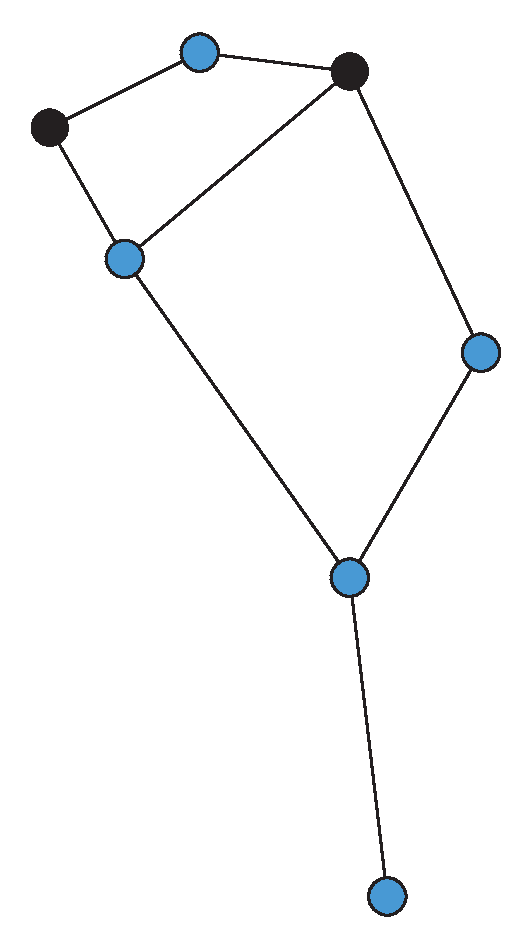
\includegraphics[width=0.20\textwidth]{./figures/subaru_ds.pdf}
&
	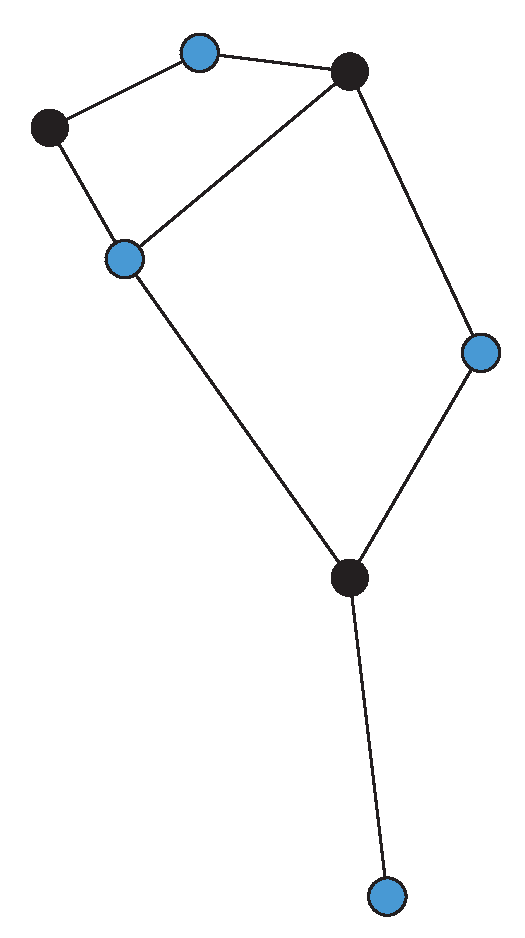
\includegraphics[width=0.20\textwidth]{./figures/subaru_mds4.pdf}
&
	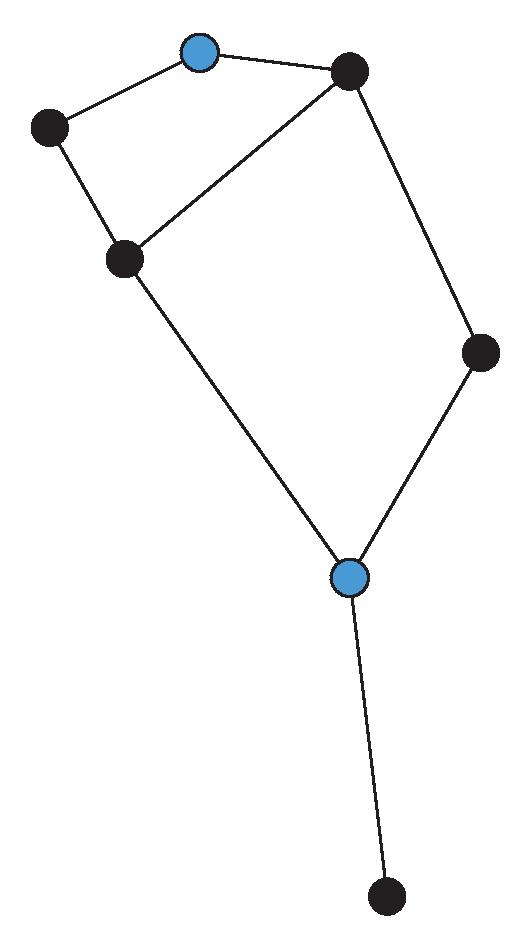
\includegraphics[width=0.20\textwidth]{./figures/subaru_mds2.pdf}\\
	\centering\bf{a} & \centering\bf{b} & \centering\bf{c}
	\end{tabular}
	\caption{Example of different dominating sets for $G(V, E)$. Vertices in the dominating set $D$ are highlighted in blue. {\bf{a)}} A dominating set of $G$ with domination number $\overline{\overline{D}} = 5$. {\bf{b)}} A minimal dominating set of $G$ with domination number of $\overline{\overline{D}} = 4$. We note that $D$ is also the maximum independent set of $G$. {\bf{c)}} The minimum dominating set of $G$ with domination number of $\overline{\overline{D}} = 2$.}
	\label{fig:dominating_sets}
\end{figure*}

For general graphs, existing "classical" algorithms either find minimal solutions in exponential time $\sim O( 1.5^n)$ \cite{Fomin2009, vanRooij2009} or approximate solutions in polynomial time. For example, greedy algorithms locally optimize decisions about which nodes to add to the dominating set.
Thus one is guaranteed to find a dominating set but not necessarily a MDS.
We demonstrate an example greedy algorithm in figure Fig.~\ref{fig:mds-greedy}.
\begin{figure*}
	\centering
	\begin{tabular}{p{0.22\textwidth}p{0.22\textwidth}p{0.22\textwidth}p{0.22\textwidth}}
	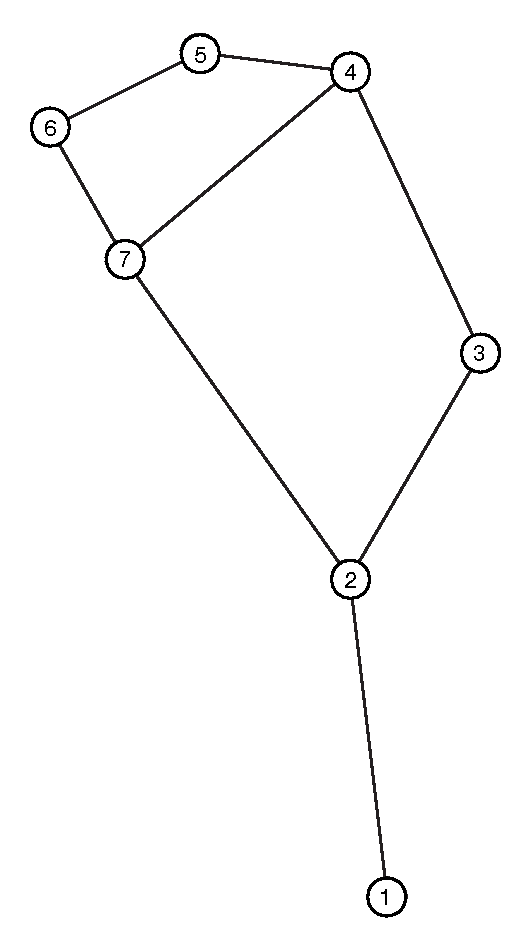
\includegraphics[width=0.20\textwidth]{./figures/greedy-1.pdf}
&
	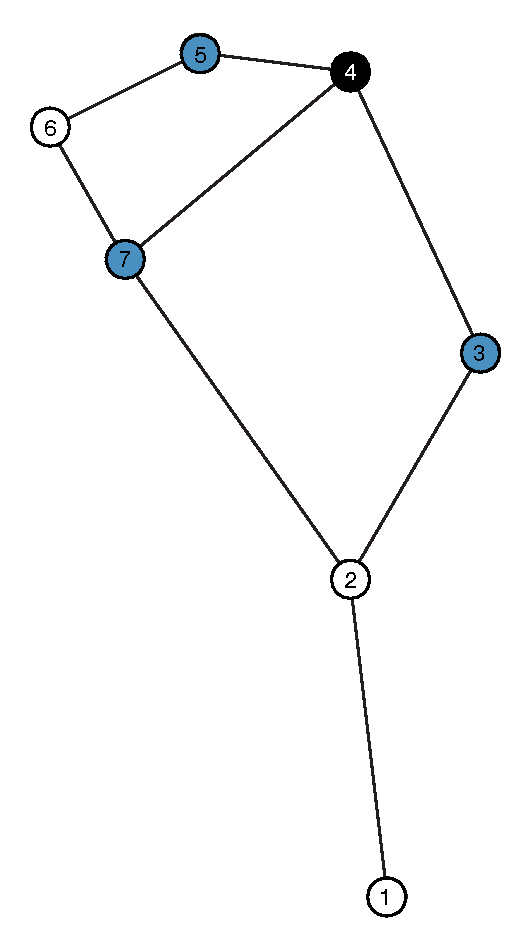
\includegraphics[width=0.20\textwidth]{./figures/greedy-2.pdf}
&
	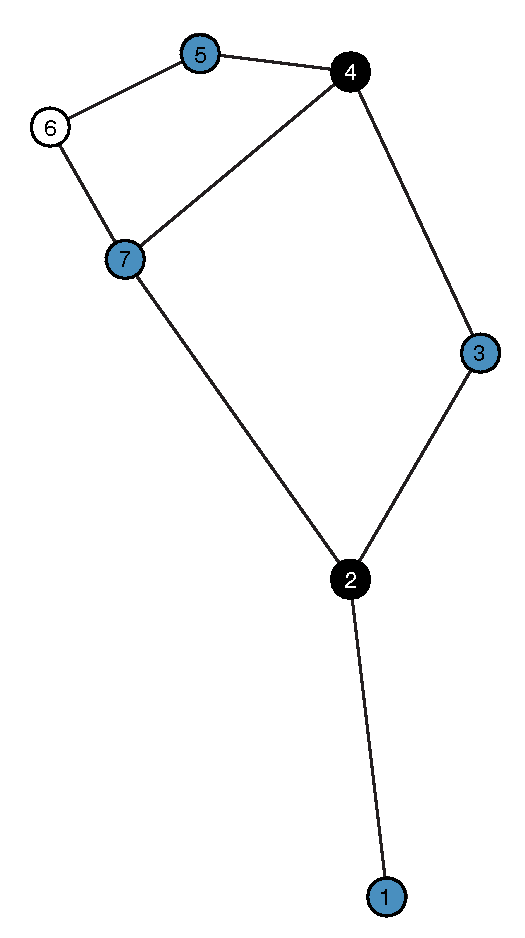
\includegraphics[width=0.20\textwidth]{./figures/greedy-3.pdf}
&
	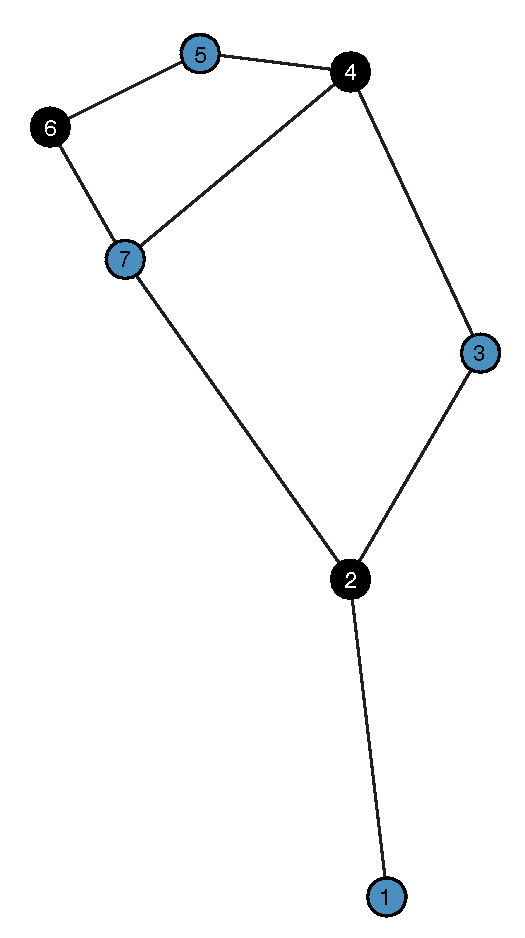
\includegraphics[width=0.20\textwidth]{./figures/greedy-4.pdf}\\
	\centering\bf{a} & \centering\bf{b} & \centering\bf{c} & \centering\bf{d}
	\end{tabular}
	\caption{
		Example of greedy MDS algorithm:
		The algorithm iteratively adds vertices to the dominating set (black nodes) such that newly added nodes are maximally unconnected (white nodes).
		Connected nodes are neighbors of the DS (turquoise) or already in the DS.
		In (a), one finds three unconnected nodes [(2), (4), (7)] which are adjacent to three unconnected nodes each.
		In the first step $a\to b$, randomly the node (4) is picked.
		In (b), one has two unconnected choices [(1), (2)] with each adjacent to another unconnected node.
		After randomly selecting (2) when going from $b \to c$, only one unconnected node is remaining (6).
		The found solution is a (minimal) dominating set but not a MDS.
		To find the MDS using this greedy algorithm, the first node choice must be either (2) or (5).
	}
	\label{fig:mds-greedy}
\end{figure*}

\subsubsection{Minimum Dominating Set}
The solution to the minimum independent set can be expressed as an integer optimization problem given by,
\begin{align}
f(x) = &\min(\sum_{\nu \in V} \psi^x_{\nu}),\\
\textrm{subject to} \quad & \psi^x_{\nu} + \sum_{\mu \in \mathit{N}(\nu)} \psi^x_{\mu} \geq 1,\\
& \psi^x_{\nu} \in \{0, 1\}
\end{align}
where the dimension of the dependent variable $x$ is the number of vertices $\overline{\overline{V}}$.
The problem minimizes the number of vertices in $D$ with a binary variable $\psi^x$ encoded by a single qubit, subject to the constraint that at least one vertex in $\mathit{N}(\nu)$ is in $D$. For each vertex in $V$ we introduce slack variables $s_{\nu} = T^s_{\nu \alpha} \psi^s_{\alpha}$ to encode the inequality constraint such that
\begin{align}
f(x) = &\min(\sum_{\nu\in V} \psi^x_{\nu}),\\
\textrm{subject to} \quad & \psi^x_{\nu} + J_{\nu \mu} \psi^x_{\mu}- T^s_{\nu \alpha} \psi^s_{\alpha}  - 1 = 0,\\
& \psi_{\nu} \in \{0, 1\},\\
& 0 \leq s_{\nu} \leq |\mathrm{N}(\nu)|\\
& s_{\nu} \in \mathbb{Z},
\end{align}
where the nearest-neighbor sum is expressed by $J$ (symmetric and zero diagonal), the adjacency matrix for $G$.
The algorithm uses $N_q = \overline{\overline{V}} + \sum_{\nu \in V} \log_2 \mathit(N(\nu))$ qubits---$\overline{\overline{V}}$ qubits to encode the vertices and another $\sum_{\nu \in V} \log_2 \mathit(N(\nu))$ qubits to embed the slack variables. Therefore, the embedding at worse scales with $\overline{\overline{V}} \log_2 |\overline{\overline{V}}|$ qubits for fully connected graphs.

The target Hamiltonian can be written in the matrix form
\begin{widetext}
\begin{align}
E = &
\begin{pmatrix}
\Psi^x & \Psi^s
\end{pmatrix}
\begin{pmatrix}
\mathbbm{1} + p\left[J^T J + J^T + J - 2 \mathrm{Diag}_{\psi^x}(|J|) - \mathbbm{1} \right] & - p(\mathbbm{1}+J^T)T^s\\
- p{T^s}^T(\mathbbm{1}+J)& p\left[{T^s}^T T^s + 2\mathrm{Diag}_{\psi^s}(|T^s|)\right]
\end{pmatrix}
\begin{pmatrix}
\Psi^x\\ \Psi^s
\end{pmatrix} + p \overline{\overline{V}}
\label{eq:matrix_form}
\end{align}
\end{widetext}
where $ |M| \equiv \sum_{\nu} M_{\nu \mu}$.

\section{DISCUSSION}

\subsection{Finding the Dominating Set with a Quantum Annealer}
\label{sec:discussion:qa}
\begin{figure}[b]
	\centering
		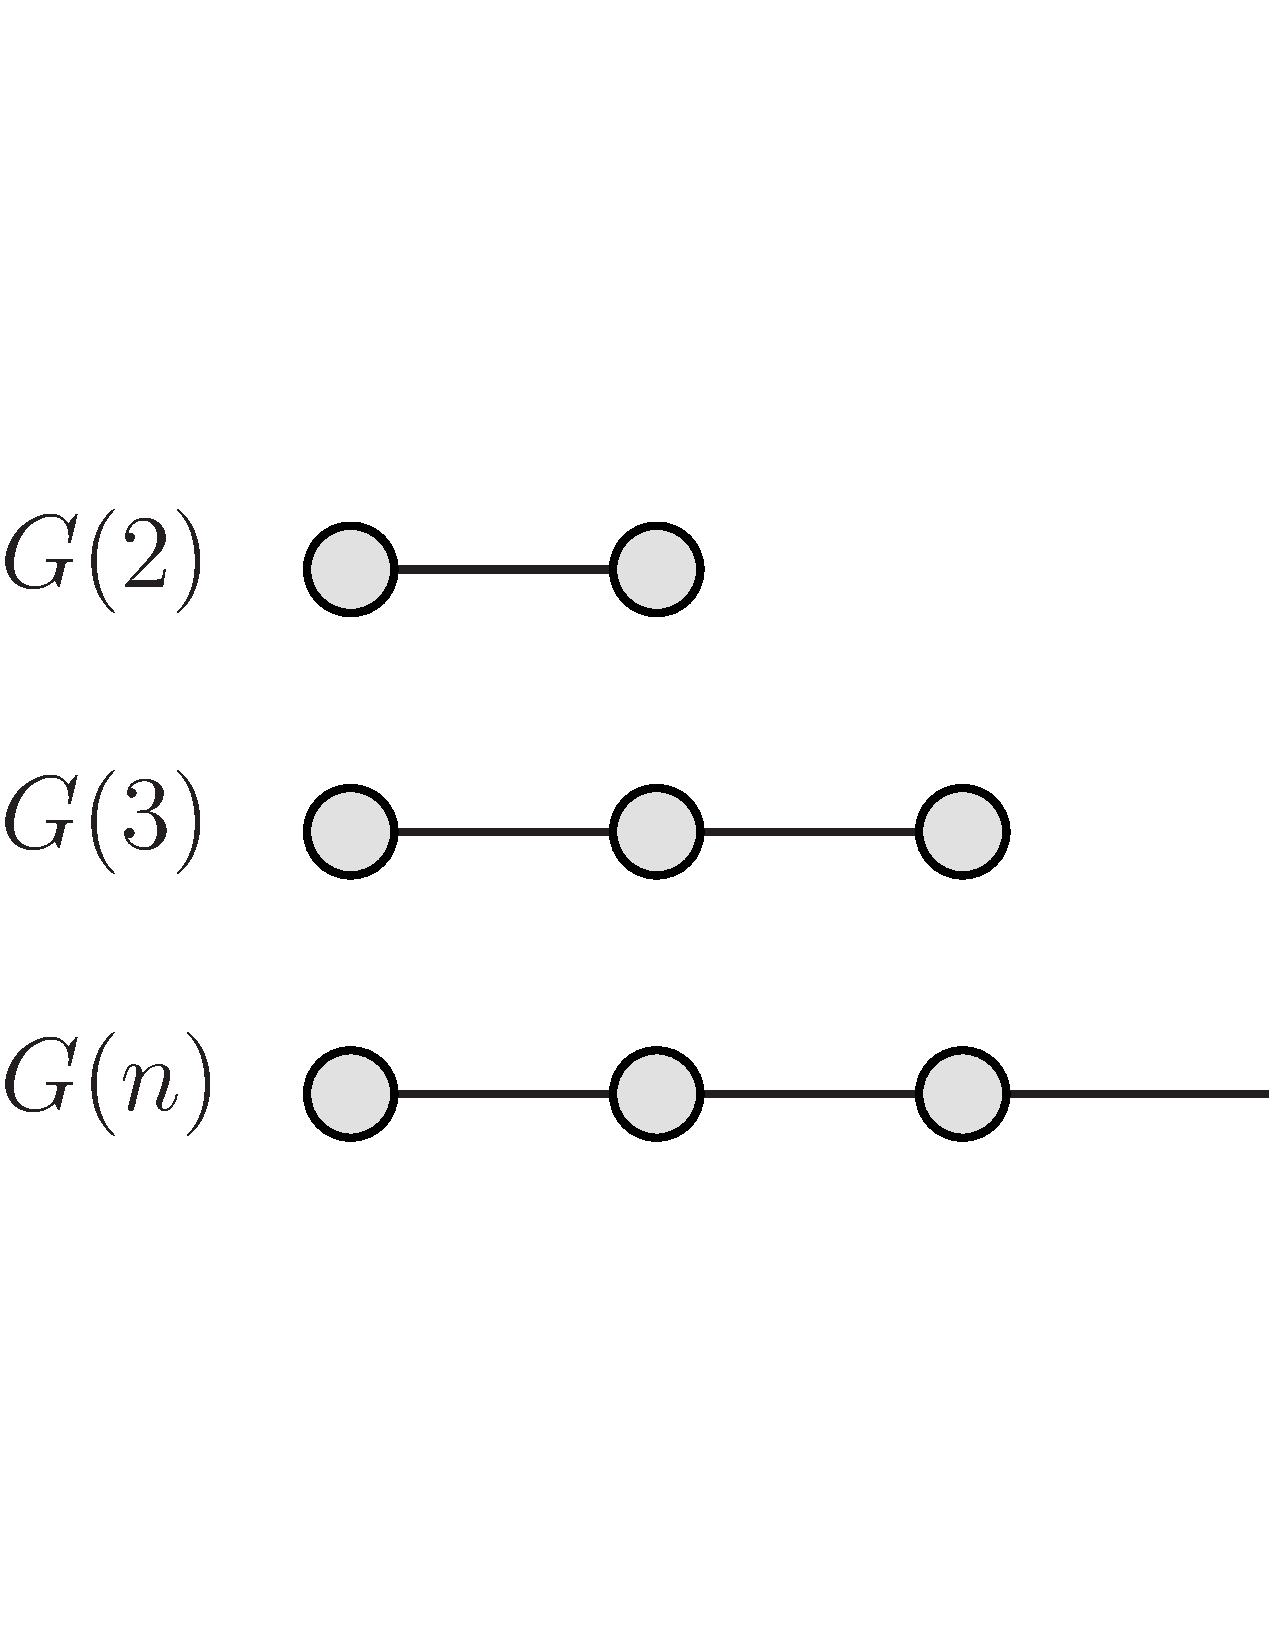
\includegraphics[width=0.5\columnwidth]{./figures/linear_crop.pdf}
	\caption{Linear graphs $G(n)$ used in this study. Nodes denote vertices of the graphs and lines are undirected edges.}
	\label{fig:linear}
\end{figure}

We demonstrate the proposed algorithm in order to obtain the MDS on a series of linear graphs $G(n)$ as shown in Fig.~\ref{fig:linear}. This type of graph is chosen because the small number of nearest-neighbor connections is more efficiently embedded into the chimera graph allowing for scaling plots to be generated when using a DWave quantum annealer. Additionally the MDS solution is known analytically, and contains both unique and degenerate solutions. In particular, the domination number for $G(n)$ is $\lceil n/3 \rceil$ while the number of MDS solutions for $n$ vertices is
\begin{align}
&1 &&\textrm{if} && n\textrm{ mod }3=0,\nonumber \\
&2\lfloor n/3 \rfloor + 1 && \textrm{if}&& n\textrm{ mod }3=1,\nonumber \\
&\lfloor n/3 \rfloor + 2 && \textrm{if} && n \textrm{ mod }3 = 2,
\end{align}
and gives the probability of randomly guessing the MDS of $G(n)$.

\begin{figure}[b]
	\centering
	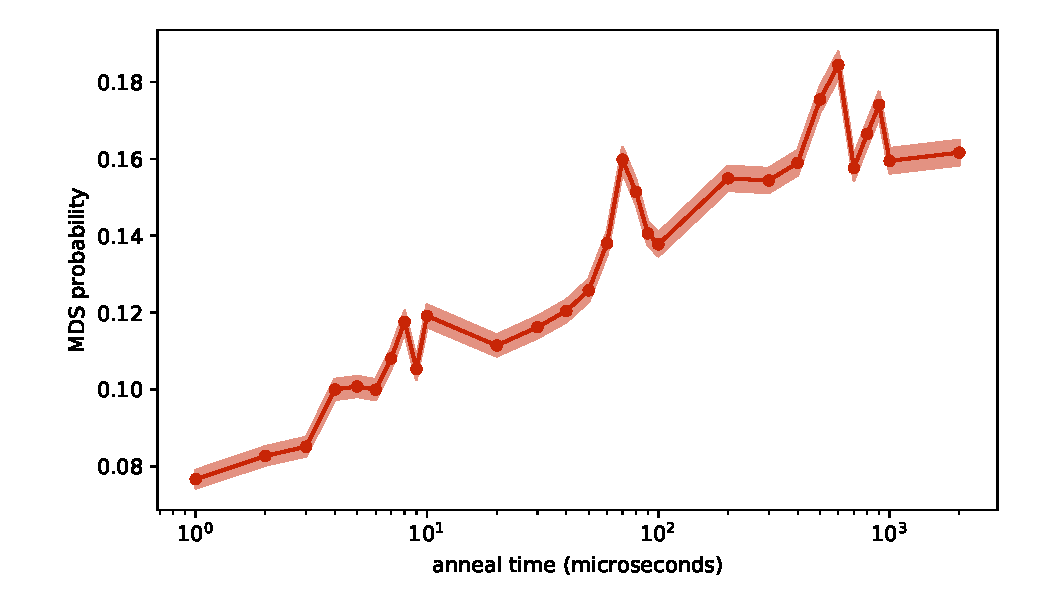
\includegraphics[width=\columnwidth]{./figures/anneal_time_scaling.pdf}
	\caption{Probability of finding the MDS for $G(6)$ as a function of total annealing time.}
	\label{fig:at_scale}
\end{figure}

For the following studies, we perform experiments on the \texttt{DW\_2000Q\_5} solver. The annealing time is optimized to 600$\mu$s after performing a study on the $G(6)$ graph as shown in Fig.~\ref{fig:at_scale}. In Fig.~\ref{fig:baseline}, we show results from the baseline experiment, without modification to the default DWave annealing schedule, and observe improvement over random guessing. However, the experiment results reflect the same degeneracy structure as random guessing, and scale exponentially poorly for larger number of vertices $n$. We explore one avenue towards improving the experiment results by introducing per-qubit annealing offsets into the time evolution.

\begin{figure}
	\centering
	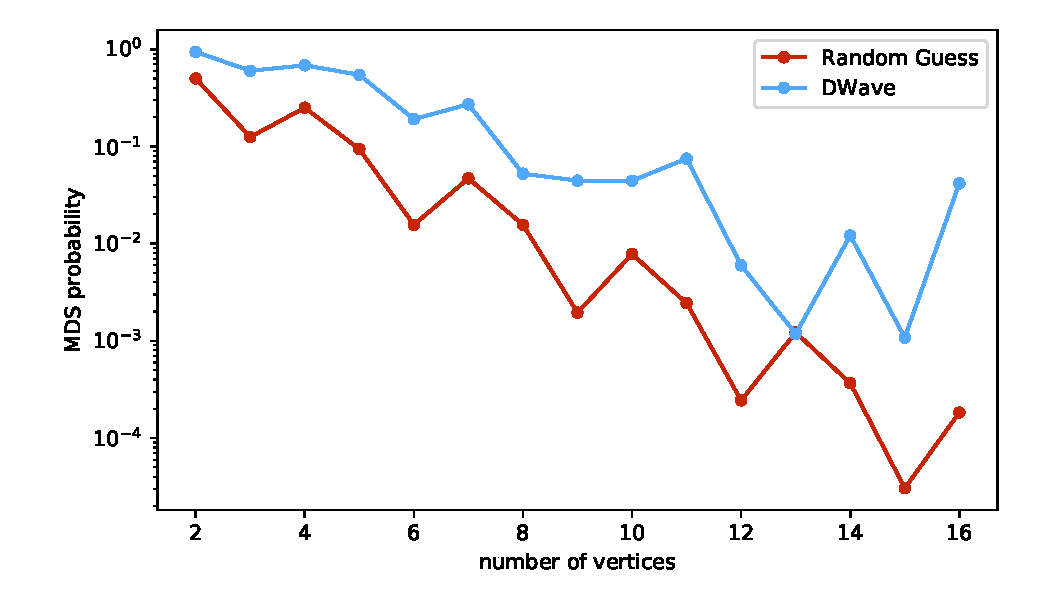
\includegraphics[width=\columnwidth]{./figures/scaling_baseline.pdf}
	\caption{Baseline result of DWave (blue) compared to random guessing (red). The jagged nature of random guessing reflects the degeneracy of the ground state.}
	\label{fig:baseline}
\end{figure}

\subsubsection{Modified annealing schedule}

In quantum annealing, the ground state of the problem Hamiltonian is obtained from the evolution of a time-dependent Hamiltonian,
\begin{equation}
H(s) = A(s) H^{\textrm{init}} + B(s) H^{\textrm{problem}}, \label{eq:tdhamiltonian}
\end{equation}
where $H^\textrm{init}=\sum_i\sigma^x_i$ on the DWave, and $H^\textrm{problem}$ is given by Eq.~(\ref{eq:matrix_form}) for the MDS application. The variable $s\in [0, 1]$ is the normalized annealing time and is allowed to vary between 1$\mu s$ to 2$ms$ on the DWave. On DWave solvers, annealing offsets effectively advance or delay the annealing schedule of individual qubits. In Fig.~\ref{fig:anneal_schedule}, the default DWave annealing schedule is shown in addition to the effects of applying positive and negative offsets. Note that due to the way the offsets are implemented on the hardware level, systematic errors are introduced since the initial and final values of $A(s)$ and $B(s)$ will differ for qubits with different offsets. Fig.~\ref{fig:anneal_schedule} shows the maximum offset that we use for the study, which translates to approximately (due to non-linearity) a 5\% advancement (blue) or delay (red) in the schedule.

\begin{figure}[b]
	\centering
	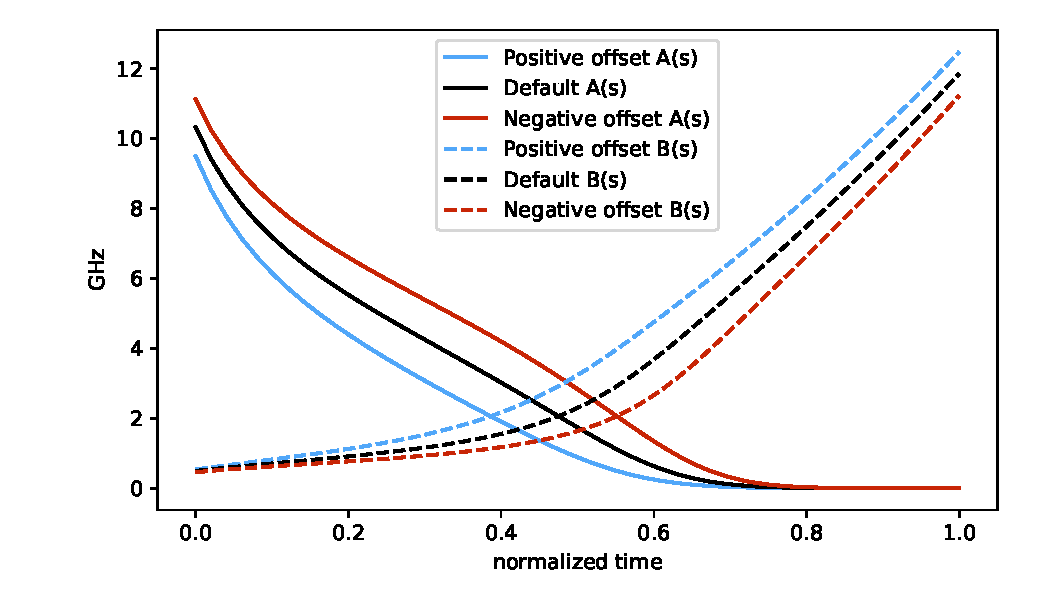
\includegraphics[width=\columnwidth]{./figures/anneal_schedule.pdf}
	\caption{asdf}
	\label{fig:anneal_schedule}
\end{figure}

The motivation behind implementing per-qubit level offsets is rooted in the hypothesis that as the problem Hamiltonian is turned on, the system in general will exhibit more disorder. We define disorder by first recasting the QUBO into its Ising form such that the problem Hamiltonian has the form
\begin{equation}
H^{\textrm{Ising}} = \sum_{ij} J_{ij} \sigma^z_i \sigma^z_j + \sum_i h_i \sigma^z_i,
\end{equation}
and recognize that in the limit where $h_i$ is randomly drawn from a Bernoulli distribution we recover the spin-glass model. The spin-glass model enters its glassy state when $|h_i|$ is large, and as a consequence, the wavefunction experiences many-body localization effects, the many-body analogue of Anderson Localization.

Following this logic, we split the qubits into two groups depending on the value of $h_i$ relative to $(\textrm{max}|\{h\}| - \textrm{min}|\{h\}|) / 2$ given the set of external magnetic fields $\{h\}$ defined by a specific problem. We then symmetrically offset the two groups of qubits over a total range between 0\% and 10\% (-5\% to +5\%). The results of this study is shown in Fig.~\ref{fig:dwave_offset}.

\begin{figure}[b]
	\centering
	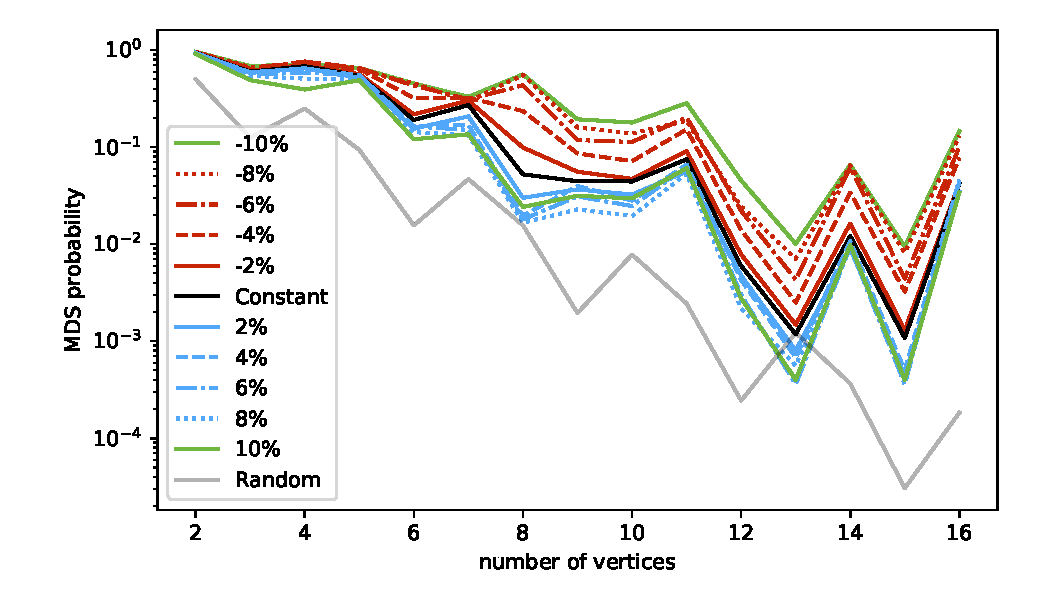
\includegraphics[width=\columnwidth]{./figures/scaling_comparison_all.pdf}
	\caption{The legend labels the total range of the symmetric offset employed. A positive range indicates that the group of qubits with small values of $|h_i|$ are advanced (qubits with large values of $|h_i|$ are equivalently delayed), and vice versa for results labeled with a negative range.}
	\label{fig:dwave_offset}
\end{figure}

Finally, we note that due to the inherent variance in performance when using different physical qubits, for each graph, we perform the offset study on the same physical qubits. Additionally, the largest offset ranges sampled are at the limits of the hardware capabilities of the DWave annealer.

We observe from Fig.~\ref{fig:dwave_offset} that advancing qubits subject to \textit{larger} final external magnetic fields yields approximately an order of magnitude improvement over the baseline results at the largest offset range. In contrast advancing qubits with weaker magnetic fields consistently hurts the performance of the annealer. This result is surprising in light of the expectation from many-body localization. We provide an explanation of this surprising result by simulating the annealing process of the annealer which are discussed in the following sections.

\subsection{Simulation Results}

In order to understand the effects of annealing offsets, we simulate the annealing process on 5 qubits for a $G(2)$ graph embedded in chimera topography. In order to shorten the simulation time, we resample the DWave with a total annealing time of 1 $\mu s$. The resulting ground state probability as a function of offset measured over 200,000 observations is shown in Fig.~\ref{fig:dwave1us} (Top).

\begin{figure}
	\centering
	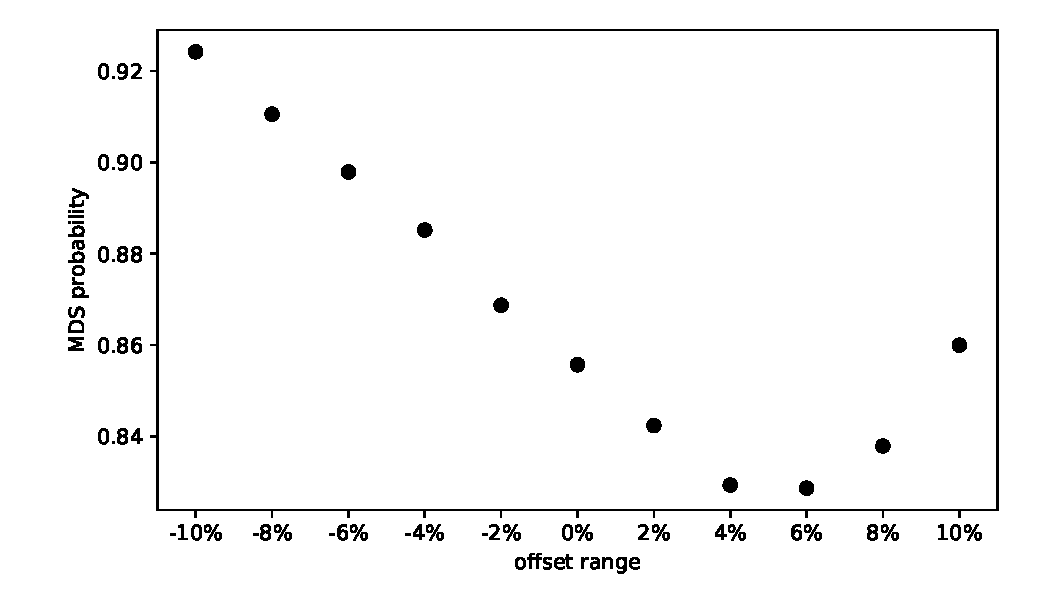
\includegraphics[width=\columnwidth]{./figures/dwave1us.pdf}
	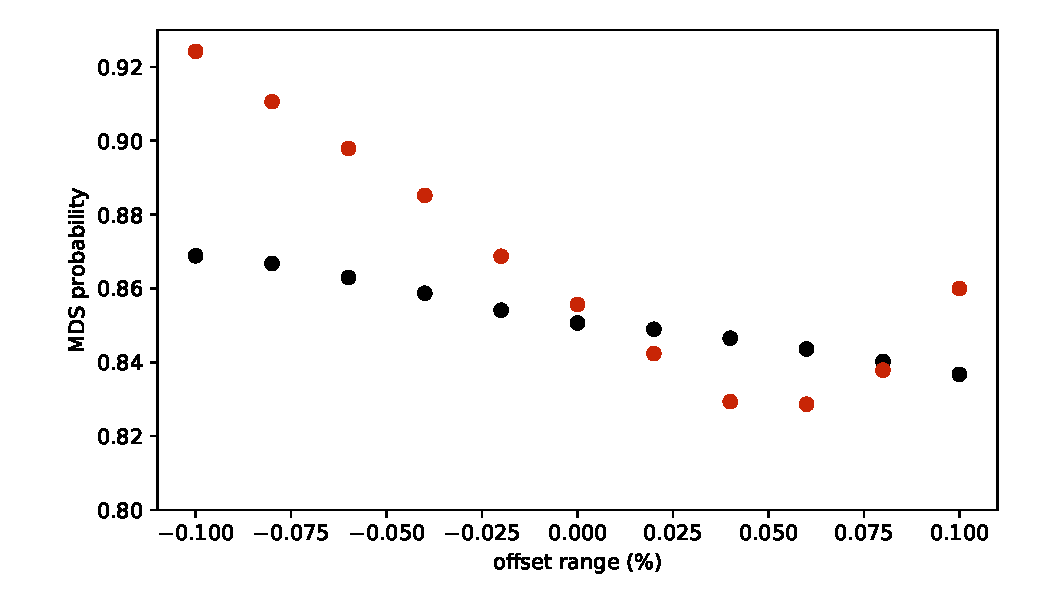
\includegraphics[width=\columnwidth]{./figures/sim_deco.pdf}
	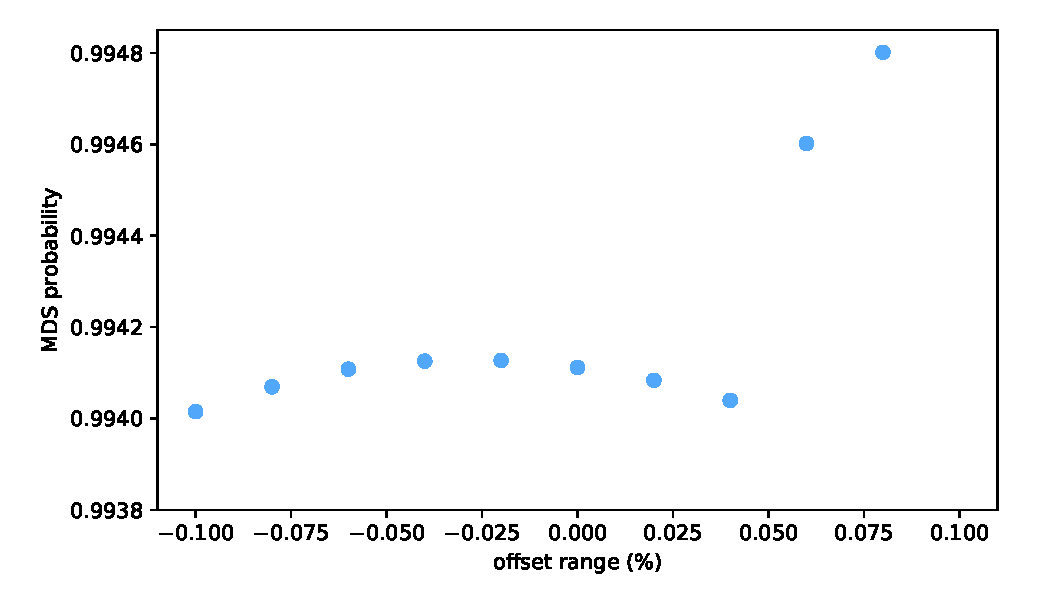
\includegraphics[width=\columnwidth]{./figures/sim_nodeco.pdf}
	\caption{ (Top) The probability of finding the MDS for $G(2)$ from DWave. The machine parameters are identical to Sec.~\ref{sec:discussion:qa} with the exception of shortening the total annealing time to 1 $\mu s$ to accommodate reasonable simulation times. (Middle) Result from simulation with decoherence and (Bottom) simulation without decoherence. In both simulations, at +10\% offset, the probability of finding the ground state vanishes. The red simulation points are not present in the DWave result.}
	\label{fig:dwave1us}
\end{figure}

For the simulation, the QUBO is obtained from the output of the DWave such that the same embedding is used. The time-dependence is obtained by solving the Lindblad equation subject to the DWave annealing schedule with offsets allowing us to incorporate a decoherence model in our simulation. The details of the Lindbladian are given in Sec.~\ref{sec:methods:lindblad}. Following Ref.~\cite{}, we fix the temperature of the simulation to 15 milliKelvins to reflect the reported operating temperature of the DWave. Due to the small size of the problem, the minimum gap to the second excited state (first non-degenerate state) of the time-dependent Hamiltonian is approximately 2 Kelvins as shown in Fig.~\ref{fig:spectrum}. As a result, the DWave operates at effectively zero-temperature for this example problem.

We then set an effective $T_1$ coherence time to 20 $ns$ in order to match the DWave probability of finding the MDS of $G(2)$ at approximately 86\%. A detailed study of $T_1$ is given in Sec.~\ref{sec:methods:deco}. We emphasize that the effective coherence time is much longer than the single qubit coherence time of 0.5 $ns$ reported by DWave, while still being orders of magnitude shorter than the total anneal time. The simulation and the experiment however, both are able to recover the ground state with high probability regardless, and exemplifies the robustness of quantum annealing.

\begin{figure}
	\centering
	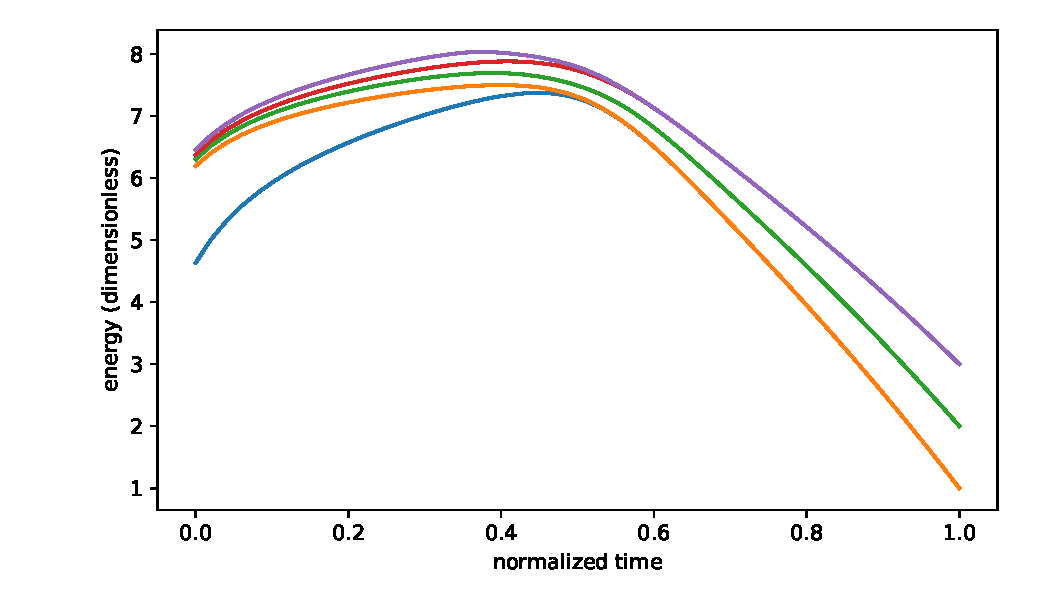
\includegraphics[width=\columnwidth]{./figures/spectrum.pdf}
	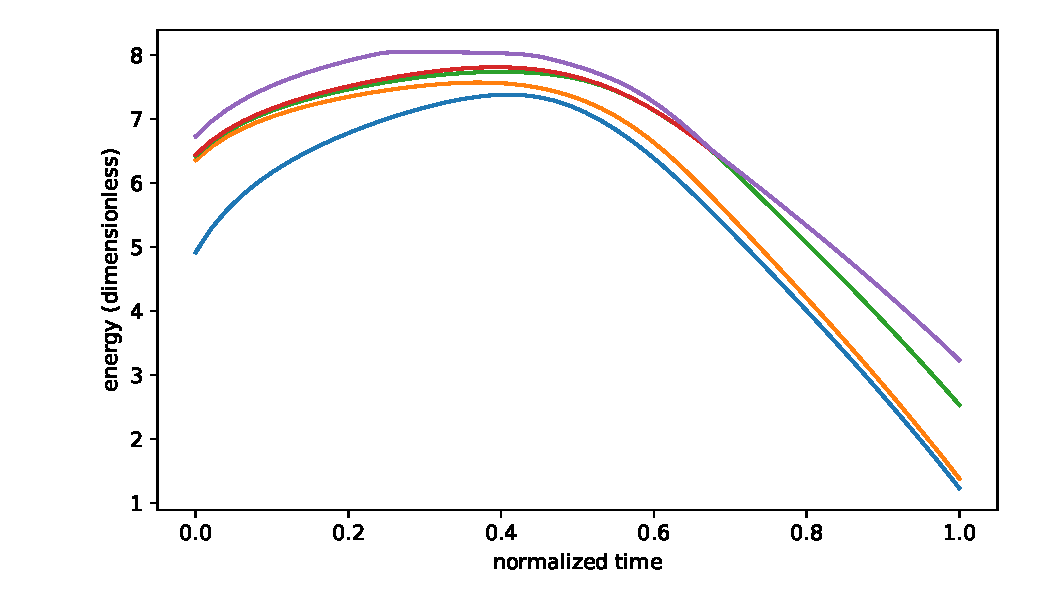
\includegraphics[width=\columnwidth]{./figures/spectrum_offset.pdf}
	\caption{The energy spectrum of the first 5 states of the time-dependent Hamiltonian (Top) without annealing offsets and (Bottom) -10\% annealing offset. The spectrum in dimensionless units at the end of the anneal is an integer spectrum and correspond to the number of vertices in the dominating set. For $G(2)$, the MDS has 1 vertex. Annealing offsets lift the ground-state degeneracy.}
	\label{fig:spectrum}
\end{figure}

The probability of finding the MDS from the simulation with and without decoherence are given in Fig.~\ref{fig:dwave_offset} (Middle) and (Bottom). We observe that with decoherence, the simulation captures the rough features of the experiment, including a steady improvement for negative offsets, and similar non-linear behavior at positive offsets. Additionally, the range of probabilities in the simulation non-trivially match the range observed in experiment. In contrast, simulations without decoherence exemplify the opposite behavior with respect to offsets, in line with expectation from many-body localization. Therefore, the simulation provides evidence in relating the improvement seen on the DWave to the effects of decoherence rather than many-body localization, while for idealized annealing, the effects of many-body localization become important.

In both simulations, the system experience a relatively large jump in probability, at -10\% and +30\% respectively. For the simulation with decoherence, this behavior is inconsistent with experiment.  {\color{red} eh.. guess a reason?} Additionally, both simulations experience vanishing probability at +10\% offset. This behavior is expected to happen eventually in experiment as well when the two sets of qubits become too aggressively staggered and effectively decouple. The simulation however, incorrectly predicts when the decoupling happens.

\subsection{Decoherence and Many-Body Localization}

We provide further evidence of the competing effects between decoherence and many-body localization in this section.

Intuitively, we want the system to explore a larger state space to increase the probability for the system to reach the final ground state. That is, we want the system to have ergodicity in order to avoid MBL. On the other hand, decoherence in the hardware leads to the loss of quantum information. It is therefore desirable to minimize the effect of relaxation. The interplay between these two competing effects can be observed by looking at the time-dependent probability of reaching the final ground state, and the mutual information. The mutual information is defined as $I(A:B)=S(\rho_A)+S(\rho_B)-S(\rho_{A,B})$, which quantifies how many bits of quantum information is communicated between partition $A$ and partition $B$ of the total system. $S(\rho)=-\mbox{Tr}\rho \log_2 \rho$ is the von Neumann entropy of density matrix $\rho$. {\color{blue} $\rho_{A,B}$ is the density matrix for the total system. $\rho_{A}=\mbox{Tr}_{B} (\rho_{A,B})$ is the reduced density matrix for the subsystem A.}

\begin{figure*}
	\centering
	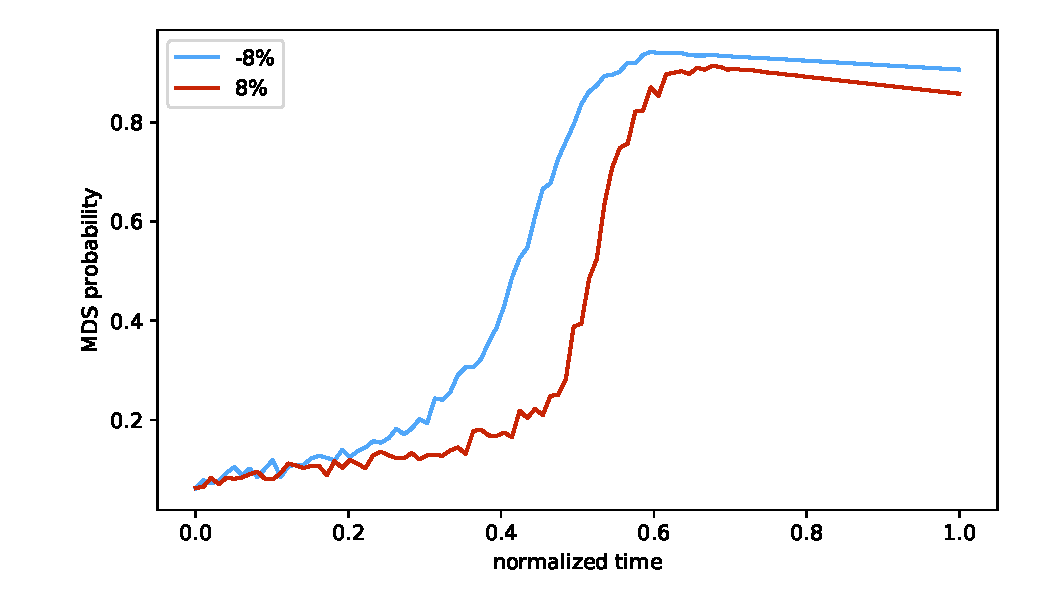
\includegraphics[width=\columnwidth]{./figures/full_prob_deco.pdf}
	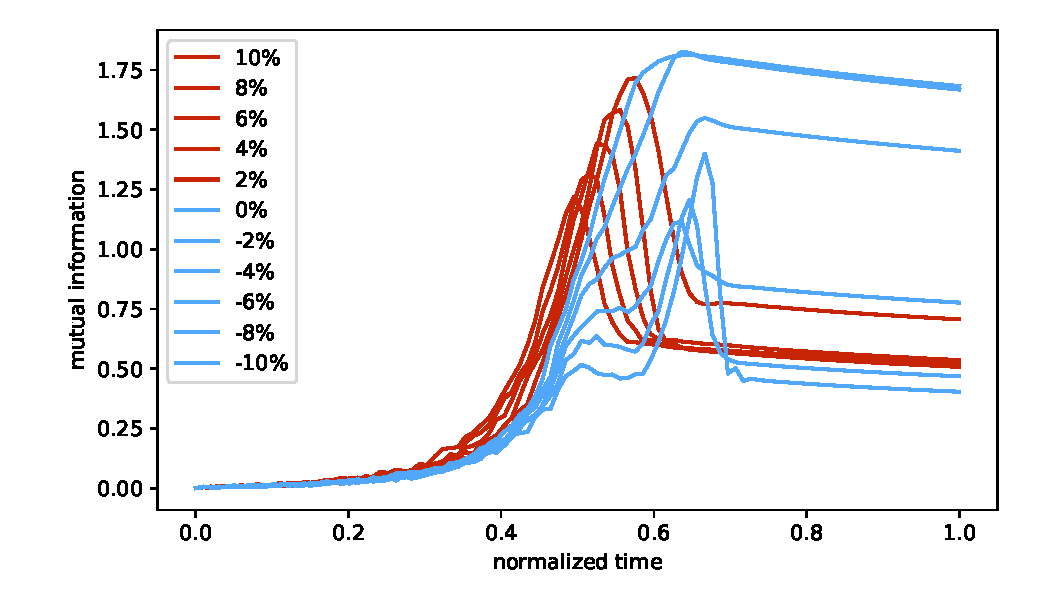
\includegraphics[width=\columnwidth]{./figures/mutual_info_deco.pdf}
	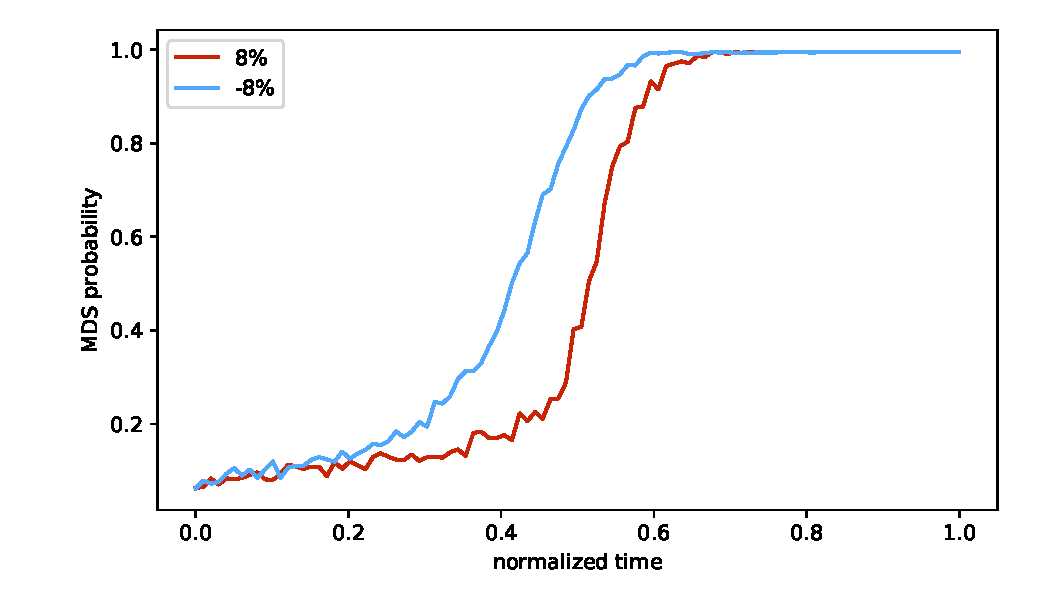
\includegraphics[width=\columnwidth]{./figures/full_prob_nodeco.pdf}
	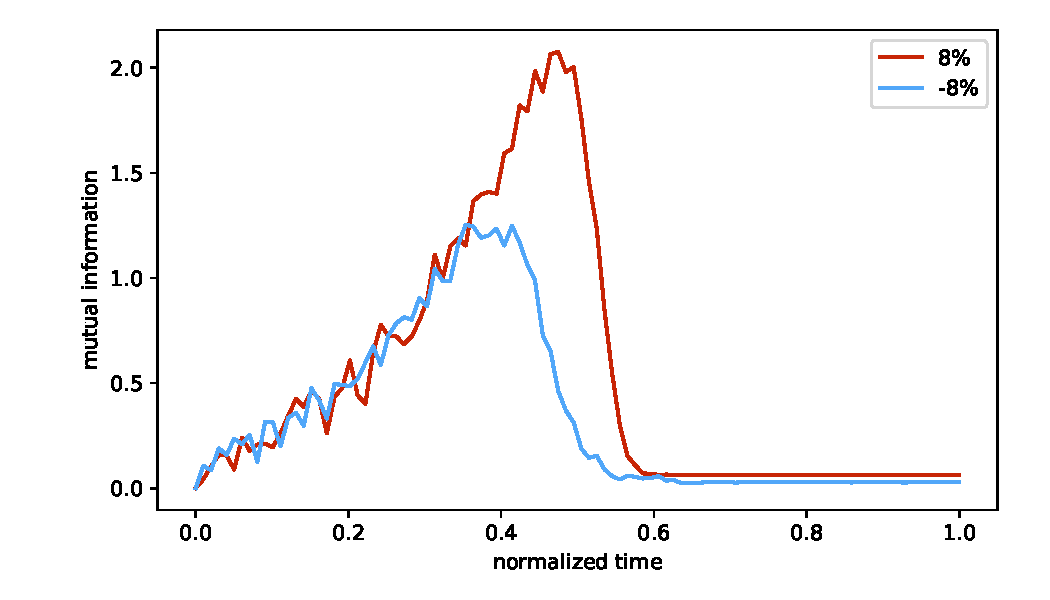
\includegraphics[width=\columnwidth]{./figures/mutual_info_nodeco.pdf}
	\caption{(Left) The time-dependent probability of resolving the ground state and (Right) the corresponding mutual information. (Top) Simulation with decoherence included and (Bottom) without decoherence.}
	\label{fig:prob_mi}
\end{figure*}

From Fig.~\ref{fig:prob_mi} we observe that when the anneal schedule is modified to delay stronger external magnetic fields, the phase transition is delayed, yielding larger mutual information, and in turn probes a larger state space. This observation is independent of the effects of decoherence, and only relies on delaying the phase transition later in the annealing process. It then follows that the effects of decoherence is in competition with delocalization because the system is required to exhibit its quantum mechanical nature for longer. In contrast, if the phase transition is advanced, effects of decoherence are more suppressed since the system freezes to its classical solution earlier in the annealing process and {\color{blue}become unaffected by dephasing.} This phenomena is demonstrated by the left panels in Fig.~\ref{fig:prob_mi} where in the case of decoherence, the schedule which delays the phase transition consistently underperforms the (bahhh help me word this. top one the red is always below blue, the bottom one, the red crosses the blue after the phase transition).

Things to do:

Compute dwave mutual information

Study ground state degeneracy by plotting distribution of states.

\section{METHODS}
\subsection{Simulation Details}
\subsubsection{The Lindblad Equation}
\label{sec:methods:lindblad}
Say what the simulator is solving

{\color{blue}


To solve for time evolution dynamics of quantum annealing including thermal and the decoherence effects, we solve for the master equation in Lindblad form
\begin{align}
\partial_t \rho (t) =  \frac{-i}{\hbar} [H(t) , \rho(t)] + \sum_j (2L_j \rho(t) L_j^\dagger - \{ L^\dagger_j L_j, \rho(t) \}) ,
\end{align}
where $\rho (t)$ is the density matrix at time $t$. $H(t)$ is the time-dependent Hamiltonian 
\begin{align}
\label{eq:annealH}
 H_{anneal}(t)&  =  - \sum_i  A_i(t)\sigma^x_i & \notag \\ 
 +&  \sum_{i>j} \sqrt{B_{i}(t)B_{j}(t)} J_{ij} \sigma^z_i \sigma^z_j +\sum_i B_{i}(t) h_i \sigma^z_i  ,&
\end{align}
where $A_i(t)$ and $B_{i}(t)$ are site-dependent annealing schedule functions. The site dependency takes into account of the annealing offset. $[,]$ denotes the Lie bracket. $L_j$ are the Lindblad operators for decoherence. $\{, \}$ denotes the anti-commutator. In this study we only include a minimal model for decoherence, i.e., the amplitude damping for non-interacting qubits. The Lindblad operator is $L_j=\sqrt{\gamma} \sigma^{+}_j$ for $h_j>0$ and $L_j=\sqrt{\gamma} \sigma^{-}_j$ for $h_j<0$, where $\gamma = 1/T_1$ is the decoherence rate for relaxation time $T_1$. For simplicity we assume all qubits having the same relaxation time. The initial condition is the Gibbs canonical ensemble
\begin{equation}
\rho (0) =  \frac{e^{-\beta H(0)}}{\mbox{Tr}[e^{-\beta H(0)}]} ,
\end{equation}
where $\beta$ is the inverse temperature.
The probability to get the ground state at measurement is
\begin{align}
P =  \mbox{Tr} \{  \rho (t) \pi_{\mbox{gnd}} \}  ,
\end{align}
where the projection operator onto the degenerated ground states subspace is defined as $\pi_{\mbox{gnd}}=\sum_{i\in G} |\mbox{gnd}_i\rangle \langle \mbox{gnd}_i| $. Here $\{ | \mbox{gnd}_i \rangle | i \in G \}$ forms an orthonormal basis for the degenerated ground states subspace, i.e., $\langle \mbox{gnd}_j | \mbox{gnd}_i \rangle = \delta_{ij}$.





}

With anneal offsets

\subsubsection{Other Simulation Details}
Temperature
Initial wave function choices
RK tolerance

\subsubsection{Decoherence Time}
\label{sec:methods:deco}

Mention long coherence time asymptote to right value.

Scan coherence time, match to DWave.

Some more discussion about short coherence time and why it makes sense?

Travis said: Regarding T1 << T effecting the state at time T, I am thinking more about the point that the very short T1 dephasing time has the effect of quenching any coherence. In this regard, a very short T1 is pushing the systems toward a classical annealing model. The absence of any dephasing is then the best-case quantum annealing model. Consequently, the difference in outcome would trace back to this coherence being present. 

\begin{figure}
	\centering
	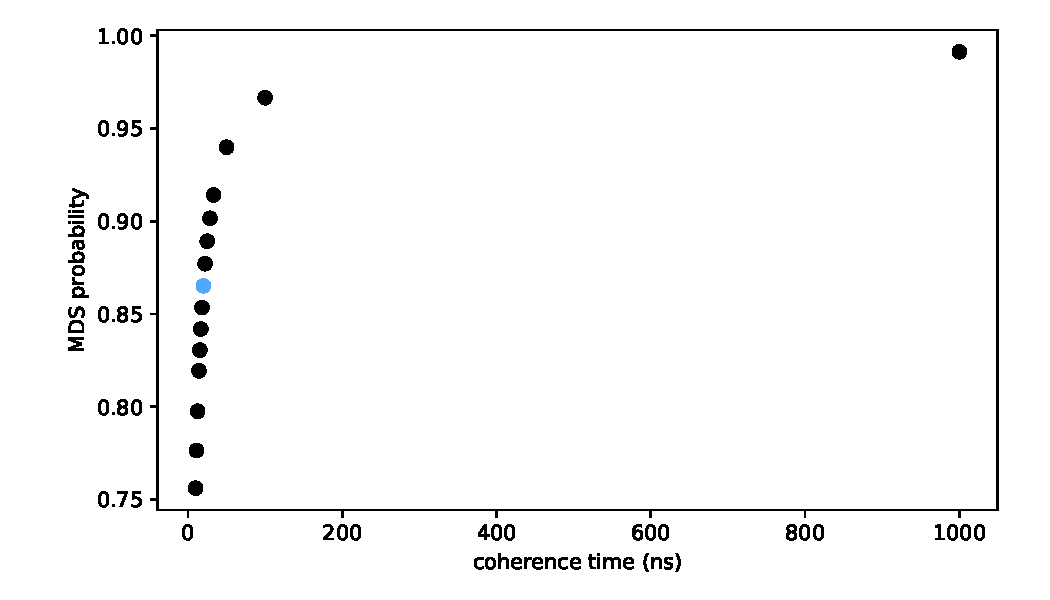
\includegraphics[width=\columnwidth]{./figures/coherence.pdf}
	\caption{asdf}
	\label{fig:prob_mi}
\end{figure}

\section{DATA AVAILABILITY}
	
Link to GitHub.

\section{ACKNOWLEDGEMENTS}

We thank x, y, z...

\section{AUTHOR CONTRIBUTIONS}

...

\section{ADDITIONAL INFORMATION}

\textbf{Competing Interests:} The authors declare no competing interests.

\bibliography{qilp}

\end{document}
